% Options for packages loaded elsewhere
\PassOptionsToPackage{unicode}{hyperref}
\PassOptionsToPackage{hyphens}{url}
%
\documentclass[
]{article}
\usepackage{amsmath,amssymb}
\usepackage{lmodern}
\usepackage{iftex}
\ifPDFTeX
  \usepackage[T1]{fontenc}
  \usepackage[utf8]{inputenc}
  \usepackage{textcomp} % provide euro and other symbols
\else % if luatex or xetex
  \usepackage{unicode-math}
  \defaultfontfeatures{Scale=MatchLowercase}
  \defaultfontfeatures[\rmfamily]{Ligatures=TeX,Scale=1}
\fi
% Use upquote if available, for straight quotes in verbatim environments
\IfFileExists{upquote.sty}{\usepackage{upquote}}{}
\IfFileExists{microtype.sty}{% use microtype if available
  \usepackage[]{microtype}
  \UseMicrotypeSet[protrusion]{basicmath} % disable protrusion for tt fonts
}{}
\makeatletter
\@ifundefined{KOMAClassName}{% if non-KOMA class
  \IfFileExists{parskip.sty}{%
    \usepackage{parskip}
  }{% else
    \setlength{\parindent}{0pt}
    \setlength{\parskip}{6pt plus 2pt minus 1pt}}
}{% if KOMA class
  \KOMAoptions{parskip=half}}
\makeatother
\usepackage{xcolor}
\usepackage[margin=1in]{geometry}
\usepackage{color}
\usepackage{fancyvrb}
\newcommand{\VerbBar}{|}
\newcommand{\VERB}{\Verb[commandchars=\\\{\}]}
\DefineVerbatimEnvironment{Highlighting}{Verbatim}{commandchars=\\\{\}}
% Add ',fontsize=\small' for more characters per line
\usepackage{framed}
\definecolor{shadecolor}{RGB}{248,248,248}
\newenvironment{Shaded}{\begin{snugshade}}{\end{snugshade}}
\newcommand{\AlertTok}[1]{\textcolor[rgb]{0.94,0.16,0.16}{#1}}
\newcommand{\AnnotationTok}[1]{\textcolor[rgb]{0.56,0.35,0.01}{\textbf{\textit{#1}}}}
\newcommand{\AttributeTok}[1]{\textcolor[rgb]{0.77,0.63,0.00}{#1}}
\newcommand{\BaseNTok}[1]{\textcolor[rgb]{0.00,0.00,0.81}{#1}}
\newcommand{\BuiltInTok}[1]{#1}
\newcommand{\CharTok}[1]{\textcolor[rgb]{0.31,0.60,0.02}{#1}}
\newcommand{\CommentTok}[1]{\textcolor[rgb]{0.56,0.35,0.01}{\textit{#1}}}
\newcommand{\CommentVarTok}[1]{\textcolor[rgb]{0.56,0.35,0.01}{\textbf{\textit{#1}}}}
\newcommand{\ConstantTok}[1]{\textcolor[rgb]{0.00,0.00,0.00}{#1}}
\newcommand{\ControlFlowTok}[1]{\textcolor[rgb]{0.13,0.29,0.53}{\textbf{#1}}}
\newcommand{\DataTypeTok}[1]{\textcolor[rgb]{0.13,0.29,0.53}{#1}}
\newcommand{\DecValTok}[1]{\textcolor[rgb]{0.00,0.00,0.81}{#1}}
\newcommand{\DocumentationTok}[1]{\textcolor[rgb]{0.56,0.35,0.01}{\textbf{\textit{#1}}}}
\newcommand{\ErrorTok}[1]{\textcolor[rgb]{0.64,0.00,0.00}{\textbf{#1}}}
\newcommand{\ExtensionTok}[1]{#1}
\newcommand{\FloatTok}[1]{\textcolor[rgb]{0.00,0.00,0.81}{#1}}
\newcommand{\FunctionTok}[1]{\textcolor[rgb]{0.00,0.00,0.00}{#1}}
\newcommand{\ImportTok}[1]{#1}
\newcommand{\InformationTok}[1]{\textcolor[rgb]{0.56,0.35,0.01}{\textbf{\textit{#1}}}}
\newcommand{\KeywordTok}[1]{\textcolor[rgb]{0.13,0.29,0.53}{\textbf{#1}}}
\newcommand{\NormalTok}[1]{#1}
\newcommand{\OperatorTok}[1]{\textcolor[rgb]{0.81,0.36,0.00}{\textbf{#1}}}
\newcommand{\OtherTok}[1]{\textcolor[rgb]{0.56,0.35,0.01}{#1}}
\newcommand{\PreprocessorTok}[1]{\textcolor[rgb]{0.56,0.35,0.01}{\textit{#1}}}
\newcommand{\RegionMarkerTok}[1]{#1}
\newcommand{\SpecialCharTok}[1]{\textcolor[rgb]{0.00,0.00,0.00}{#1}}
\newcommand{\SpecialStringTok}[1]{\textcolor[rgb]{0.31,0.60,0.02}{#1}}
\newcommand{\StringTok}[1]{\textcolor[rgb]{0.31,0.60,0.02}{#1}}
\newcommand{\VariableTok}[1]{\textcolor[rgb]{0.00,0.00,0.00}{#1}}
\newcommand{\VerbatimStringTok}[1]{\textcolor[rgb]{0.31,0.60,0.02}{#1}}
\newcommand{\WarningTok}[1]{\textcolor[rgb]{0.56,0.35,0.01}{\textbf{\textit{#1}}}}
\usepackage{longtable,booktabs,array}
\usepackage{calc} % for calculating minipage widths
% Correct order of tables after \paragraph or \subparagraph
\usepackage{etoolbox}
\makeatletter
\patchcmd\longtable{\par}{\if@noskipsec\mbox{}\fi\par}{}{}
\makeatother
% Allow footnotes in longtable head/foot
\IfFileExists{footnotehyper.sty}{\usepackage{footnotehyper}}{\usepackage{footnote}}
\makesavenoteenv{longtable}
\usepackage{graphicx}
\makeatletter
\def\maxwidth{\ifdim\Gin@nat@width>\linewidth\linewidth\else\Gin@nat@width\fi}
\def\maxheight{\ifdim\Gin@nat@height>\textheight\textheight\else\Gin@nat@height\fi}
\makeatother
% Scale images if necessary, so that they will not overflow the page
% margins by default, and it is still possible to overwrite the defaults
% using explicit options in \includegraphics[width, height, ...]{}
\setkeys{Gin}{width=\maxwidth,height=\maxheight,keepaspectratio}
% Set default figure placement to htbp
\makeatletter
\def\fps@figure{htbp}
\makeatother
\setlength{\emergencystretch}{3em} % prevent overfull lines
\providecommand{\tightlist}{%
  \setlength{\itemsep}{0pt}\setlength{\parskip}{0pt}}
\setcounter{secnumdepth}{-\maxdimen} % remove section numbering
\newlength{\cslhangindent}
\setlength{\cslhangindent}{1.5em}
\newlength{\csllabelwidth}
\setlength{\csllabelwidth}{3em}
\newlength{\cslentryspacingunit} % times entry-spacing
\setlength{\cslentryspacingunit}{\parskip}
\newenvironment{CSLReferences}[2] % #1 hanging-ident, #2 entry spacing
 {% don't indent paragraphs
  \setlength{\parindent}{0pt}
  % turn on hanging indent if param 1 is 1
  \ifodd #1
  \let\oldpar\par
  \def\par{\hangindent=\cslhangindent\oldpar}
  \fi
  % set entry spacing
  \setlength{\parskip}{#2\cslentryspacingunit}
 }%
 {}
\usepackage{calc}
\newcommand{\CSLBlock}[1]{#1\hfill\break}
\newcommand{\CSLLeftMargin}[1]{\parbox[t]{\csllabelwidth}{#1}}
\newcommand{\CSLRightInline}[1]{\parbox[t]{\linewidth - \csllabelwidth}{#1}\break}
\newcommand{\CSLIndent}[1]{\hspace{\cslhangindent}#1}
\ifLuaTeX
  \usepackage{selnolig}  % disable illegal ligatures
\fi
\IfFileExists{bookmark.sty}{\usepackage{bookmark}}{\usepackage{hyperref}}
\IfFileExists{xurl.sty}{\usepackage{xurl}}{} % add URL line breaks if available
\urlstyle{same} % disable monospaced font for URLs
\hypersetup{
  pdftitle={ASSIGNMENT 4},
  pdfauthor={Luke Syverson},
  hidelinks,
  pdfcreator={LaTeX via pandoc}}

\title{ASSIGNMENT 4}
\author{Luke Syverson}
\date{2023-04-23}

\begin{document}
\maketitle

\hypertarget{markdown-basics}{%
\section{Markdown Basics}\label{markdown-basics}}

\hypertarget{favorite-foods}{%
\subsection{Favorite Foods}\label{favorite-foods}}

\begin{enumerate}
\def\labelenumi{\arabic{enumi})}
\tightlist
\item
  Beef Steak
\item
  Fish
\item
  Sourdough Bread \#\# Images
  \includegraphics{~/School/Github Desktop/dsc520/completed/assignment04/plots}
  All Cases (Log Plot) \#\# Add a Quote \textgreater{} ``Out of all the
  things I have lost, I miss my mind the most.'' -- Mark Twain
\end{enumerate}

\hypertarget{add-an-equation}{%
\subsection{Add an Equation}\label{add-an-equation}}

\[\frac{1+ \sqrt5}{2}\] \#\# Add a Footnote

This is a footnote\footnote{This is the above footnote description.}.

\hypertarget{add-citations}{%
\subsection{Add Citations}\label{add-citations}}

\begin{itemize}
\tightlist
\item
  R for Everyone (Lander (2014))
\item
  Discovering Statistics Using R (Field, Miles, and Field (2012))
\end{itemize}

\hypertarget{inline-code}{%
\section{Inline Code}\label{inline-code}}

\hypertarget{ny-times-covid-19-data}{%
\subsection{NY Times COVID-19 Data}\label{ny-times-covid-19-data}}

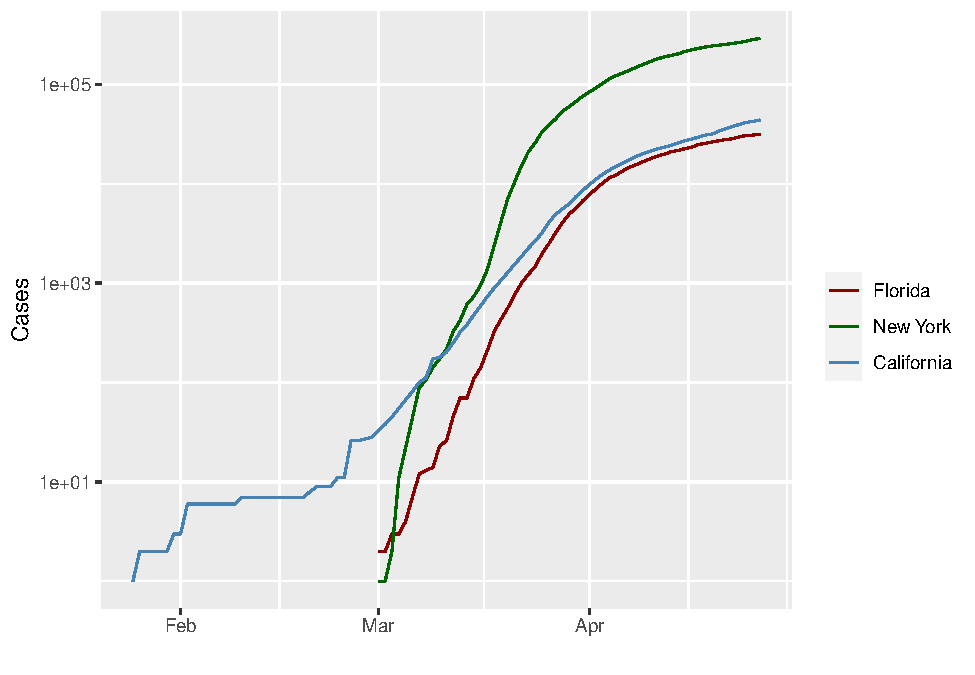
\includegraphics{assignment_04_SyversonLuke_files/figure-latex/unnamed-chunk-2-1.pdf}
\#\# R4DS Height vs Earnings
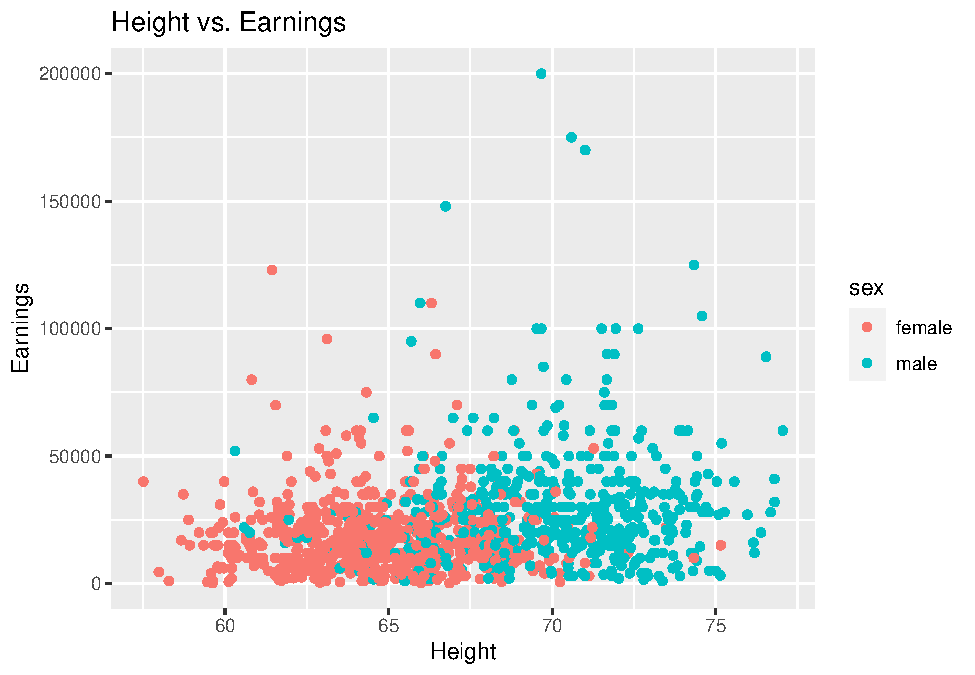
\includegraphics{assignment_04_SyversonLuke_files/figure-latex/unnamed-chunk-3-1.pdf}
\# Tables

\begin{Shaded}
\begin{Highlighting}[]
\NormalTok{name }\OtherTok{\textless{}{-}} \FunctionTok{c}\NormalTok{(}\StringTok{"Aragon"}\NormalTok{, }\StringTok{"Bilbo"}\NormalTok{, }\StringTok{"Frodo"}\NormalTok{, }\StringTok{"Galadriel"}\NormalTok{, }\StringTok{"Sam"}\NormalTok{, }\StringTok{"Gandalf"}\NormalTok{, }\StringTok{"Legolas"}\NormalTok{, }\StringTok{"Sauron"}\NormalTok{, }\StringTok{"Gollum"}\NormalTok{)}
\NormalTok{race }\OtherTok{\textless{}{-}} \FunctionTok{c}\NormalTok{(}\StringTok{"Men"}\NormalTok{, }\StringTok{"Hobbit"}\NormalTok{, }\StringTok{"Hobbit"}\NormalTok{, }\StringTok{"Elf"}\NormalTok{, }\StringTok{"Hobbit"}\NormalTok{, }\StringTok{"Maia"}\NormalTok{, }\StringTok{"Elf"}\NormalTok{, }\StringTok{"Maia"}\NormalTok{, }\StringTok{"Hobbit"}\NormalTok{)}
\NormalTok{in\_fellowship }\OtherTok{\textless{}{-}} \FunctionTok{c}\NormalTok{(}\ConstantTok{TRUE}\NormalTok{, }\ConstantTok{FALSE}\NormalTok{, }\ConstantTok{TRUE}\NormalTok{, }\ConstantTok{FALSE}\NormalTok{, }\ConstantTok{TRUE}\NormalTok{, }\ConstantTok{TRUE}\NormalTok{, }\ConstantTok{TRUE}\NormalTok{, }\ConstantTok{FALSE}\NormalTok{, }\ConstantTok{FALSE}\NormalTok{)}
\NormalTok{ring\_bearer }\OtherTok{\textless{}{-}} \FunctionTok{c}\NormalTok{(}\ConstantTok{FALSE}\NormalTok{, }\ConstantTok{TRUE}\NormalTok{, }\ConstantTok{TRUE}\NormalTok{, }\ConstantTok{FALSE}\NormalTok{, }\ConstantTok{TRUE}\NormalTok{, }\ConstantTok{TRUE}\NormalTok{, }\ConstantTok{FALSE}\NormalTok{, }\ConstantTok{TRUE}\NormalTok{, }\ConstantTok{TRUE}\NormalTok{)}
\NormalTok{age }\OtherTok{\textless{}{-}} \FunctionTok{c}\NormalTok{(}\DecValTok{88}\NormalTok{, }\DecValTok{129}\NormalTok{, }\DecValTok{51}\NormalTok{, }\DecValTok{7000}\NormalTok{, }\DecValTok{36}\NormalTok{, }\DecValTok{2019}\NormalTok{, }\DecValTok{2931}\NormalTok{, }\DecValTok{7052}\NormalTok{, }\DecValTok{589}\NormalTok{)}
\NormalTok{characters\_df }\OtherTok{\textless{}{-}} \FunctionTok{data.frame}\NormalTok{(name, race, in\_fellowship, ring\_bearer, age)}
\end{Highlighting}
\end{Shaded}

\hypertarget{knitr-table-with-kable}{%
\subsection{Knitr Table with Kable}\label{knitr-table-with-kable}}

\begin{Shaded}
\begin{Highlighting}[]
\FunctionTok{library}\NormalTok{(stringr)}
\NormalTok{knitr}\SpecialCharTok{::}\FunctionTok{kable}\NormalTok{(characters\_df, }\AttributeTok{caption =} \StringTok{\textquotesingle{}One Ring to Rule Them All\textquotesingle{}}
\NormalTok{             , }\AttributeTok{col.names =} \FunctionTok{str\_to\_title}\NormalTok{(}\FunctionTok{gsub}\NormalTok{(}\StringTok{"\_"}\NormalTok{, }\StringTok{" "}\NormalTok{, }\FunctionTok{names}\NormalTok{(characters\_df))))}
\end{Highlighting}
\end{Shaded}

\begin{longtable}[]{@{}llllr@{}}
\caption{One Ring to Rule Them All}\tabularnewline
\toprule()
Name & Race & In Fellowship & Ring Bearer & Age \\
\midrule()
\endfirsthead
\toprule()
Name & Race & In Fellowship & Ring Bearer & Age \\
\midrule()
\endhead
Aragon & Men & TRUE & FALSE & 88 \\
Bilbo & Hobbit & FALSE & TRUE & 129 \\
Frodo & Hobbit & TRUE & TRUE & 51 \\
Galadriel & Elf & FALSE & FALSE & 7000 \\
Sam & Hobbit & TRUE & TRUE & 36 \\
Gandalf & Maia & TRUE & TRUE & 2019 \\
Legolas & Elf & TRUE & FALSE & 2931 \\
Sauron & Maia & FALSE & TRUE & 7052 \\
Gollum & Hobbit & FALSE & TRUE & 589 \\
\bottomrule()
\end{longtable}

\hypertarget{pandoc-table}{%
\subsection{Pandoc Table}\label{pandoc-table}}

\begin{Shaded}
\begin{Highlighting}[]
\FunctionTok{library}\NormalTok{(pander)}
\FunctionTok{pandoc.table}\NormalTok{(characters\_df, }\AttributeTok{style =} \StringTok{\textquotesingle{}rmarkdown\textquotesingle{}}\NormalTok{)}
\end{Highlighting}
\end{Shaded}

\begin{verbatim}
## 
## 
## |   name    |  race  | in_fellowship | ring_bearer | age  |
## |:---------:|:------:|:-------------:|:-----------:|:----:|
## |  Aragon   |  Men   |     TRUE      |    FALSE    |  88  |
## |   Bilbo   | Hobbit |     FALSE     |    TRUE     | 129  |
## |   Frodo   | Hobbit |     TRUE      |    TRUE     |  51  |
## | Galadriel |  Elf   |     FALSE     |    FALSE    | 7000 |
## |    Sam    | Hobbit |     TRUE      |    TRUE     |  36  |
## |  Gandalf  |  Maia  |     TRUE      |    TRUE     | 2019 |
## |  Legolas  |  Elf   |     TRUE      |    FALSE    | 2931 |
## |  Sauron   |  Maia  |     FALSE     |    TRUE     | 7052 |
## |  Gollum   | Hobbit |     FALSE     |    TRUE     | 589  |
\end{verbatim}

\begin{Shaded}
\begin{Highlighting}[]
\CommentTok{\# I\textquotesingle{}m not sure if this is the right way to do this, but it works!}
\end{Highlighting}
\end{Shaded}

\hypertarget{references}{%
\section*{References}\label{references}}
\addcontentsline{toc}{section}{References}

\hypertarget{refs}{}
\begin{CSLReferences}{1}{0}
\leavevmode\vadjust pre{\hypertarget{ref-field2012discovering}{}}%
Field, A., J. Miles, and Z. Field. 2012. \emph{Discovering Statistics
Using r}. SAGE Publications.
\url{https://books.google.com/books?id=wd2K2zC3swIC}.

\leavevmode\vadjust pre{\hypertarget{ref-lander2014r}{}}%
Lander, J. P. 2014. \emph{R for Everyone: Advanced Analytics and
Graphics}. Addison-Wesley Data and Analytics Series. Addison-Wesley.
\url{https://books.google.com/books?id=3eBVAgAAQBAJ}.

\end{CSLReferences}

\end{document}
